
\documentclass[letterpaper]{article}



\usepackage{times}
\usepackage{uist}
\usepackage{graphicx}

\begin{document}

% --- Copyright notice ---
\conferenceinfo{UIST'09}{October 4-7, 2009, Victoria, British Columbia, Canada}
\CopyrightYear{2009}
\crdata{978-1-60558-745-5/09/10}

% Uncomment the following line to hide the copyright notice
% \toappear{}
% ------------------------

\bibliographystyle{plain}

%\title{Standard UIST Conference Format:\\
%       Preparing Camera-Ready Submissions}
\title{Voicify: User Demonstrated Voice Interfaces}

%\author{Adam Vogel \and Arda Kara}

%%
%% Note on formatting authors at different institutions, as shown below:
%% Change width arg (currently 7cm) to parbox commands as needed to
%% accommodate widest lines, taking care not to overflow the 17.8cm line width.
%% Add or delete parboxes for additional authors at different institutions. 
%% If additional authors won't fit in one row, you can add a "\\"  at the
%% end of a parbox's closing "}" to have the next parbox start a new row.
%% Be sure NOT to put any blank lines between parbox commands!
%%

\author{
\parbox[t]{9cm}{\centering
	     {\em Adam Vogel}\\
     Computer Science Department\\
             Stanford University \\
	     av@cs.stanford.edu}
\parbox[t]{9cm}{\centering
	     {\em Arda Kara}\\
	     Computer Science Department\\
       Stanford University\\
	     ardakara@stanford.edu}
}

\maketitle

\abstract
%Although voice interfaces exist for the main functions of modern mobile phones, many community-developed 
%applications lack speech support. 
We present \emph{Voicify}, a framework for voice programming by 
demonstration which enables users to build their own speech interfaces.
The user creates their own voice interface by demonstrating a voice command with the corresponding
actions to take on the phone. The phone can then be put in a hands-free mode, where it
responds to previously programmed voice commands. 
Transparency is a key issue, and we discuss the development of a voice-only keyboard for
text entry paired with a custom screen reader for giving feedback to the user.
We conducted a user study which shows that
interfaces created using Voicify rival their touch counterparts.
However, our study also shows that most users find programming by demonstration to be
tedious, and that the natural language processing is too impoverished to be widely applicable.

\section{Introduction}
Speech interfaces have been gaining in popularity with the proliferation of mobile devices. Smartphones are
frequently used in hands-free or eyes-free contexts, such as while driving or walking. Modern phones like
the iPhone and Android phones include speech recognition and synthesis in the operating system, allowing
users to make calls and send text messages by voice. However, there is a long tail of community authored
phone applications which have no voice interface. This is a big restriction for the convenience of
hands-free users and the sight disabled. 

To address this problem, we introduce \emph{Voicify}, a framework for creating speech interfaces 
through end-user demonstration. Voicify allows a user to create voice commands for Android
applications through a ``tell and show'' interface: the user first \emph{tells} the phone what 
to do in natural language and then \emph{shows} the phone how to interpret this command.
Once the user has demonstrated commands, the phone can execute commands in a playback mode.

We further explore the efficacy of user demonstration and the usability of the resulting
interface by conducting a user study.  We \emph{voicified} a popular open-source Android todo list
application called \emph{Astrid} (CITE). Using this version of Astrid, we tested the ease and
competence of the demonstration and playback interfaces when compared to the traditional touch
interface. Our results show that the voicified interfaces are usable, with a 60\% command interpretation
success rate, but still fall below the level needed for wide usage. Our user study revealed
several weaknesses in the demonstration interaction which we implemented.

The remainder of the paper summarizes the large body of work on programming by demonstration, details
the design and implementation of Voicify, and discusses the user study.

\section{Related Work}
Some other people did this shit too!

\section{Programming by Demonstration}
The Voicify framework requires three main components: the ability to capture low-level UI events, 
an interface for recording demonstrations, and lastly the ability to playback commands for interpretation.

\subsection{UI Capture}
To record a command demonstration, Voicify requires access to the user interface actions that a user engages in.
Security restrictions on the Android platform make it impossible for a 3rd party application to capture 
touch and key events as this would enable malicious keyloggers to steal sensitive information. 
The Android Accessibility Team (CITE) confirmed that this is impossible to do without modifying the operating system.
To circumvent this problem, we chose an open-source application as a prototype, which allowed us to modify
the program source itself, thus capturing UI events within the application.

The UI design of Android still makes capturing UI events across a whole application a difficult task.
Within each activity, the interface elements, called \emph{views}, are arranged in a tree structure. When the user
touches the screen, the UI event is dispatched to the lowest element in the view tree which spans that portion of the 
screen. It is then passed up the tree, until a UI element consumes it. To capture these touch events,
we programmatically traverse the view tree and insert an invisible UI layer at each node. The UI layer
simply captures the UI interactions which pass through it.

Furthermore, some UI widgets like buttons and dialog boxes consume touch events without passing them along
to the activity in which they reside. Complicating matters, these boxes are required to be leaves
of the view tree, which doesn't allow for our trick of inserting invisible layers. To deal with these issues
we overrode the UI widget classes to capture the interactions. This required changing the UI definitions for
each of the screens to use our modified versions. This challenges our goal of making Voicify applicable to
every application but is a necessary hack for this prototype.

Lastly, each screen in an Android application is run in its own process, which pauses when switching between
screens in an application. This makes it difficult to share UI events across activities, which very naturally
happens when demonstrating some commands. To overcome this we implemented a \emph{demonstration service} which runs in the background
of the application and aggregates UI interactions across activities.

When recording UI events, we capture low-level touches. The information in touch events includes the (X,Y) coordinate
on the screen, the pressure and size, and lastly whether it is initial contact, a dragging motion, or a release.
Our various capturing shims transmit these events to the demonstration service, which associates them with the
correct command. Recording demonstrations at this low-level is the source of some errors. For instance, imagine
the user demonstrates how to click the 'save' button on a screen with a list. If the user later adds elements to the
list and tries to play back the 'save' command, the button might have moved. This is a large source of error in 
our experiments.


%TODO: figure for the demonstration service? like boxes and arrows and shit.

\subsection{Demonstration Interface}
We now describe the user demonstration interface. We modified the hard camera button on the phone to serve as the 
``Voicify button''. After loading the Astrid application, the user clicks the camera button. This pops up a small
notification which says ``Demonstration'' (Figure \ref{fig:interface}). From here the user says the command that they would like to record,
for instance ``create a new task''.
After running Google-powered speech recognition, the interface speaks back to the user what it thinks the command
is, such as ``recording command 'create a new task' ''. The phone now is in capture mode, where all subsequent
UI events are associated with this command. After executing the desired sequence of interactions, the user
again presses the camera button to signal the end of demonstration, which triggers a small popup window
to acknowledge the demonstration.

We use the hard camera-button to solve the \emph{clutching problem}, which is how to determine when a trial has ended.
We also experimented with a soft button in a context menu within the application, but users found it cumbersome
to locate, whereas the hard camera button is always there and able to be pressed by feeling alone.
An even better demonstration interface would be to always capture the audio and only record when the 
user says a key phrase. However, the current state of speech recognition is not good enough to enable this.


\begin{figure}[t]
\label{fig:interface}
\begin{center}
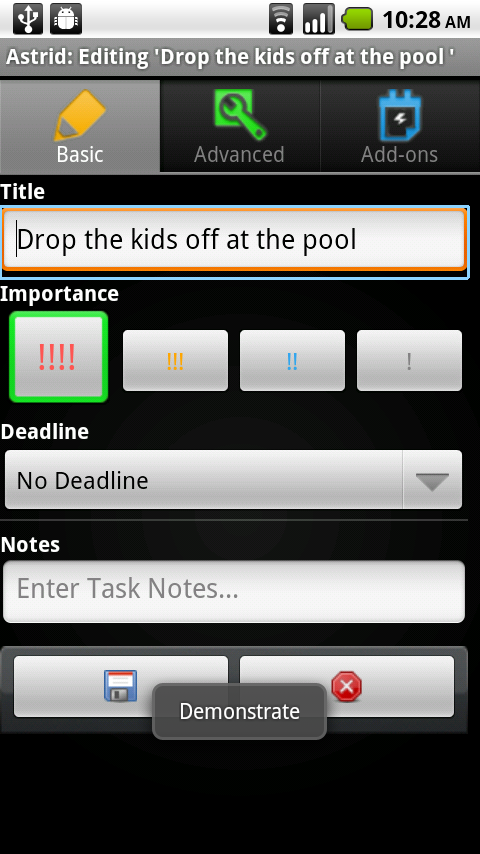
\includegraphics[scale=0.3]{fig/screenshot.png}
\end{center}
\caption{When the user presses the camera button a small UI notification appears to let them know to being demonstration.}
\end{figure}


\subsection{Playback Interface}
The Android operating system employs a sandbox-based security framework that prevents any interaction between applications. 
Each application has its own virtual machine, which makes it more difficult to implement a system-wide voice control interface without modifying the OS.
Our workaround was to use the UI testing features of the built-in unit testing tools that come with the Android SDK.
One downside of this approach is that the phone needs to be plugged into the debugging environment during testing; however, 
this didn't come up as a concern from our test users. Listening for the commands was still done on the phone, 
and the Astrid application was modified to receive a voice command upon a button press, look-up the closest matching voice command 
that it has in its database, and send the necessary UI interactions to the test suite using IPC. Our system for receiving commands used 
a word overlap index to find the closest command in its database. Just like the demonstration interface, the user would press a button 
and then utter the voice command they want to use. The phone then echoes the command that it thinks it received and carries out the 
recorded UI interactions. 
 
\begin{enumerate}
\item Screen reader
Android has a built-in screen reader tool called TalkBack that can be turned on as a system-wide setting and allows the user to get 
voice feedback from their interactions by traversing through UI elements using the d-pad on their phones (if available on the model). 
An alternative to TalkBack is a third-party open source tool called Spiel that allows per-application customization through JavaScript. 
Our system did not use either of these packages since they needed the phone's accessibility mode to be turned on, which intervened with 
custom accessibility objects that our code uses. Instead, we implemented a replacement that dispatches d-pad commands to traverse 
through visible UI elements, and simulates accessibility events to gather readable content at each step. This worked well for a uniform 
screen like the list of to-do tasks, but got in the way of user interaction in more complicated screens due to the simulated traversal. 
Therefore we only used the screen reader to read off the list of tasks.

\item Voice keyboard
We also wanted our demonstrated 

\item Natural language processing for command interpretation
\end{enumerate}

\section{Experimental Evaluation}
\subsection{Experimental Design}

\subsection{Results}

\subsection{Discussion}

\section{Conclusion and Future Work}
Potential improvements: Either infer more about UI elements (not just 
x/y coordinates, but inferring what elements the user is interacting with)
or record the context/screen the user was at during demonstration and only allow 
that command to be dispatched from the same context.


\end{document}
